\documentclass{standalone}
\usepackage{tikz}
\usetikzlibrary{patterns, positioning}
\usepackage[sfdefault]{ClearSans} %% option 'sfdefault' activates Clear Sans as the default text font
\usepackage[T1]{fontenc}

\begin{document}
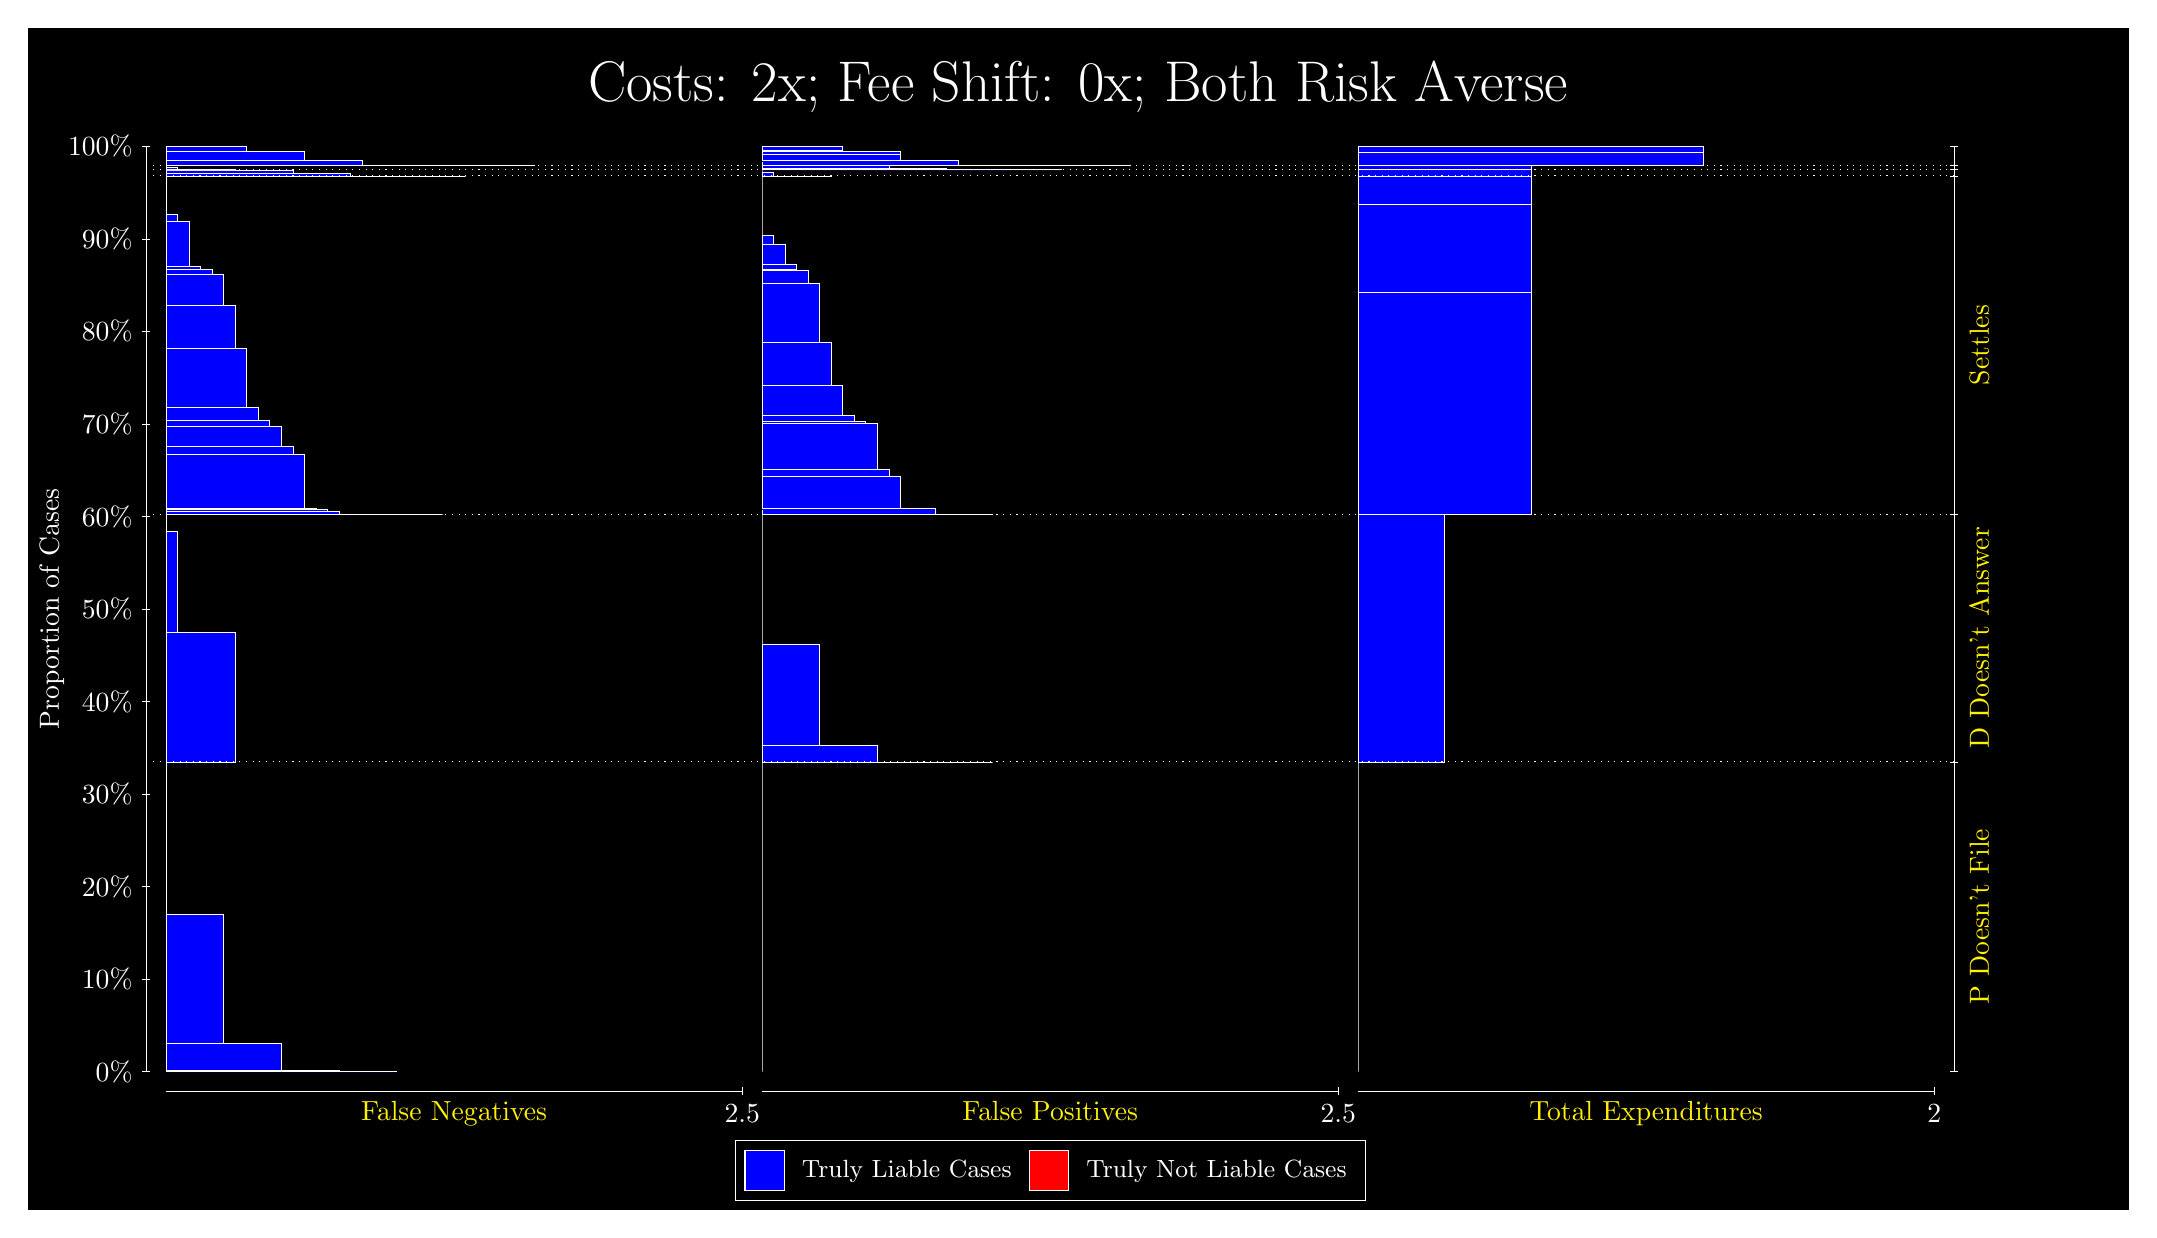
\begin{tikzpicture}
\draw[fill=black] (0,0) rectangle (26.667,15);
\draw[text=white] (0,13.5) rectangle (26.667,15) node[midway] {\huge Costs: 2x; Fee Shift: 0x; Both Risk Averse};
\draw[white, very thin] (1.5,1.75) -- (1.5,13.5);
\node[rotate=90, text=white, anchor=center] at (0.3, 7.625) {Proportion of Cases};
\draw[white, very thin] (1.45,1.75) -- (1.55,1.75);
\node[text=white, anchor=east] at (1.45, 1.75) {0\%};
\draw[white, very thin] (1.45,2.925) -- (1.55,2.925);
\node[text=white, anchor=east] at (1.45, 2.925) {10\%};
\draw[white, very thin] (1.45,4.1) -- (1.55,4.1);
\node[text=white, anchor=east] at (1.45, 4.1) {20\%};
\draw[white, very thin] (1.45,5.275) -- (1.55,5.275);
\node[text=white, anchor=east] at (1.45, 5.275) {30\%};
\draw[white, very thin] (1.45,6.45) -- (1.55,6.45);
\node[text=white, anchor=east] at (1.45, 6.45) {40\%};
\draw[white, very thin] (1.45,7.625) -- (1.55,7.625);
\node[text=white, anchor=east] at (1.45, 7.625) {50\%};
\draw[white, very thin] (1.45,8.8) -- (1.55,8.8);
\node[text=white, anchor=east] at (1.45, 8.8) {60\%};
\draw[white, very thin] (1.45,9.975) -- (1.55,9.975);
\node[text=white, anchor=east] at (1.45, 9.975) {70\%};
\draw[white, very thin] (1.45,11.15) -- (1.55,11.15);
\node[text=white, anchor=east] at (1.45, 11.15) {80\%};
\draw[white, very thin] (1.45,12.325) -- (1.55,12.325);
\node[text=white, anchor=east] at (1.45, 12.325) {90\%};
\draw[white, very thin] (1.45,13.5) -- (1.55,13.5);
\node[text=white, anchor=east] at (1.45, 13.5) {100\%};

\draw[white, very thin] (24.457,1.75) -- (24.457,13.5);
\draw[white, very thin] (24.407,1.75) -- (24.507,1.75);
\node[anchor=west] at (24.407, 1.75) {};
\draw[white, very thin] (24.407,5.6817) -- (24.507,5.6817);
\node[anchor=west] at (24.407, 5.6817) {};
\draw[white, very thin] (24.407,8.8294) -- (24.507,8.8294);
\node[anchor=west] at (24.407, 8.8294) {};
\draw[white, very thin] (24.407,13.124) -- (24.507,13.124);
\node[anchor=west] at (24.407, 13.124) {};
\draw[white, very thin] (24.407,13.204) -- (24.507,13.204);
\node[anchor=west] at (24.407, 13.204) {};
\draw[white, very thin] (24.407,13.257) -- (24.507,13.257);
\node[anchor=west] at (24.407, 13.257) {};
\draw[white, very thin] (24.407,13.5) -- (24.507,13.5);
\node[anchor=west] at (24.407, 13.5) {};

\draw[white, very thin, fill=blue] (1.75,1.75) rectangle (4.6775,1.7501);
\draw[white, very thin, fill=blue] (1.75,1.7501) rectangle (3.9457,1.7606);
\draw[white, very thin, fill=blue] (1.75,1.7606) rectangle (3.2138,2.1027);
\draw[white, very thin, fill=blue] (1.75,2.1027) rectangle (2.4819,3.7434);
\draw[white, very thin, fill=red] (1.75,3.7434) rectangle (1.75,3.7434);
\draw[white, very thin, fill=blue] (1.75,3.7434) rectangle (1.75,5.6817);
\draw[white, very thin, fill=blue] (1.75,5.6817) rectangle (2.6283,7.3327);
\draw[white, very thin, fill=blue] (1.75,7.3327) rectangle (1.8964,8.616);
\draw[white, very thin, fill=red] (1.75,8.616) rectangle (1.75,8.616);
\draw[white, very thin, fill=blue] (1.75,8.616) rectangle (1.75,8.8294);
\draw[white, very thin, fill=blue] (1.75,8.8294) rectangle (5.2631,8.8294);
\draw[white, very thin, fill=blue] (1.75,8.8294) rectangle (4.6775,8.8295);
\draw[white, very thin, fill=blue] (1.75,8.8295) rectangle (4.5312,8.8304);
\draw[white, very thin, fill=blue] (1.75,8.8304) rectangle (4.3848,8.8304);
\draw[white, very thin, fill=blue] (1.75,8.8304) rectangle (4.092,8.8307);
\draw[white, very thin, fill=blue] (1.75,8.8307) rectangle (3.9457,8.8604);
\draw[white, very thin, fill=blue] (1.75,8.8604) rectangle (3.7993,8.896);
\draw[white, very thin, fill=blue] (1.75,8.896) rectangle (3.6529,8.9037);
\draw[white, very thin, fill=blue] (1.75,8.9037) rectangle (3.5065,9.5873);
\draw[white, very thin, fill=blue] (1.75,9.5873) rectangle (3.3602,9.694);
\draw[white, very thin, fill=blue] (1.75,9.694) rectangle (3.2138,9.9497);
\draw[white, very thin, fill=blue] (1.75,9.9497) rectangle (3.0674,10.018);
\draw[white, very thin, fill=blue] (1.75,10.018) rectangle (3.0674,10.026);
\draw[white, very thin, fill=blue] (1.75,10.026) rectangle (2.921,10.191);
\draw[white, very thin, fill=blue] (1.75,10.191) rectangle (2.7746,10.941);
\draw[white, very thin, fill=blue] (1.75,10.941) rectangle (2.6283,11.484);
\draw[white, very thin, fill=blue] (1.75,11.484) rectangle (2.4819,11.87);
\draw[white, very thin, fill=blue] (1.75,11.87) rectangle (2.3355,11.942);
\draw[white, very thin, fill=blue] (1.75,11.942) rectangle (2.3355,11.942);
\draw[white, very thin, fill=blue] (1.75,11.942) rectangle (2.1891,11.976);
\draw[white, very thin, fill=blue] (1.75,11.976) rectangle (2.0428,12.551);
\draw[white, very thin, fill=blue] (1.75,12.551) rectangle (1.8964,12.643);
\draw[white, very thin, fill=red] (1.75,12.643) rectangle (1.75,12.643);
\draw[white, very thin, fill=blue] (1.75,12.643) rectangle (1.75,13.124);
\draw[white, very thin, fill=blue] (1.75,13.124) rectangle (5.5558,13.124);
\draw[white, very thin, fill=blue] (1.75,13.124) rectangle (4.8239,13.124);
\draw[white, very thin, fill=blue] (1.75,13.124) rectangle (4.092,13.154);
\draw[white, very thin, fill=blue] (1.75,13.154) rectangle (3.3602,13.202);
\draw[white, very thin, fill=blue] (1.75,13.202) rectangle (2.6283,13.204);
\draw[white, very thin, fill=red] (1.75,13.204) rectangle (1.75,13.204);
\draw[white, very thin, fill=blue] (1.75,13.204) rectangle (2.6283,13.204);
\draw[white, very thin, fill=blue] (1.75,13.204) rectangle (1.8964,13.237);
\draw[white, very thin, fill=red] (1.75,13.237) rectangle (1.75,13.237);
\draw[white, very thin, fill=blue] (1.75,13.237) rectangle (1.75,13.257);
\draw[white, very thin, fill=blue] (1.75,13.257) rectangle (6.4341,13.257);
\draw[white, very thin, fill=blue] (1.75,13.257) rectangle (5.7022,13.257);
\draw[white, very thin, fill=blue] (1.75,13.257) rectangle (4.9703,13.261);
\draw[white, very thin, fill=blue] (1.75,13.261) rectangle (4.2384,13.318);
\draw[white, very thin, fill=blue] (1.75,13.318) rectangle (3.5065,13.44);
\draw[white, very thin, fill=blue] (1.75,13.44) rectangle (2.7746,13.496);
\draw[white, very thin, fill=blue] (1.75,13.496) rectangle (2.0428,13.5);
\draw[white, very thin, fill=red] (1.75,13.5) rectangle (1.75,13.5);
\draw[white, very thin, fill=blue] (1.75,13.5) rectangle (1.75,13.5);
\draw[white, very thin, fill=red] (9.3189,1.75) rectangle (9.3189,1.75);
\draw[white, very thin, fill=blue] (9.3189,1.75) rectangle (9.3189,5.6817);
\draw[white, very thin, fill=red] (9.3189,5.6817) rectangle (12.246,5.6817);
\draw[white, very thin, fill=blue] (9.3189,5.6817) rectangle (12.246,5.6817);
\draw[white, very thin, fill=blue] (9.3189,5.6817) rectangle (11.515,5.6828);
\draw[white, very thin, fill=blue] (9.3189,5.6828) rectangle (10.783,5.8951);
\draw[white, very thin, fill=blue] (9.3189,5.8951) rectangle (10.051,7.1784);
\draw[white, very thin, fill=blue] (9.3189,7.1784) rectangle (9.3189,8.8294);
\draw[white, very thin, fill=red] (9.3189,8.8294) rectangle (12.246,8.8294);
\draw[white, very thin, fill=blue] (9.3189,8.8294) rectangle (12.246,8.8295);
\draw[white, very thin, fill=red] (9.3189,8.8295) rectangle (11.954,8.8295);
\draw[white, very thin, fill=blue] (9.3189,8.8295) rectangle (11.954,8.8295);
\draw[white, very thin, fill=red] (9.3189,8.8295) rectangle (11.661,8.8295);
\draw[white, very thin, fill=blue] (9.3189,8.8295) rectangle (11.661,8.8299);
\draw[white, very thin, fill=blue] (9.3189,8.8299) rectangle (11.515,8.899);
\draw[white, very thin, fill=red] (9.3189,8.899) rectangle (11.368,8.899);
\draw[white, very thin, fill=blue] (9.3189,8.899) rectangle (11.368,8.8994);
\draw[white, very thin, fill=blue] (9.3189,8.8994) rectangle (11.222,8.9019);
\draw[white, very thin, fill=red] (9.3189,8.9019) rectangle (11.075,8.9019);
\draw[white, very thin, fill=blue] (9.3189,8.9019) rectangle (11.075,9.3102);
\draw[white, very thin, fill=blue] (9.3189,9.3102) rectangle (10.929,9.4025);
\draw[white, very thin, fill=blue] (9.3189,9.4025) rectangle (10.783,9.977);
\draw[white, very thin, fill=blue] (9.3189,9.977) rectangle (10.636,10.012);
\draw[white, very thin, fill=red] (9.3189,10.012) rectangle (10.49,10.012);
\draw[white, very thin, fill=blue] (9.3189,10.012) rectangle (10.49,10.012);
\draw[white, very thin, fill=blue] (9.3189,10.012) rectangle (10.49,10.083);
\draw[white, very thin, fill=blue] (9.3189,10.083) rectangle (10.344,10.47);
\draw[white, very thin, fill=blue] (9.3189,10.47) rectangle (10.197,11.013);
\draw[white, very thin, fill=blue] (9.3189,11.013) rectangle (10.051,11.763);
\draw[white, very thin, fill=blue] (9.3189,11.763) rectangle (9.9044,11.928);
\draw[white, very thin, fill=blue] (9.3189,11.928) rectangle (9.758,11.935);
\draw[white, very thin, fill=blue] (9.3189,11.935) rectangle (9.758,12.004);
\draw[white, very thin, fill=blue] (9.3189,12.004) rectangle (9.6116,12.259);
\draw[white, very thin, fill=blue] (9.3189,12.259) rectangle (9.4652,12.366);
\draw[white, very thin, fill=blue] (9.3189,12.366) rectangle (9.3189,13.124);
\draw[white, very thin, fill=red] (9.3189,13.124) rectangle (10.197,13.124);
\draw[white, very thin, fill=blue] (9.3189,13.124) rectangle (10.197,13.125);
\draw[white, very thin, fill=blue] (9.3189,13.125) rectangle (9.4652,13.174);
\draw[white, very thin, fill=blue] (9.3189,13.174) rectangle (9.3189,13.204);
\draw[white, very thin, fill=red] (9.3189,13.204) rectangle (13.125,13.204);
\draw[white, very thin, fill=blue] (9.3189,13.204) rectangle (13.125,13.204);
\draw[white, very thin, fill=blue] (9.3189,13.204) rectangle (12.393,13.204);
\draw[white, very thin, fill=blue] (9.3189,13.204) rectangle (11.661,13.224);
\draw[white, very thin, fill=blue] (9.3189,13.224) rectangle (10.929,13.257);
\draw[white, very thin, fill=blue] (9.3189,13.257) rectangle (10.197,13.257);
\draw[white, very thin, fill=red] (9.3189,13.257) rectangle (14.003,13.257);
\draw[white, very thin, fill=blue] (9.3189,13.257) rectangle (14.003,13.257);
\draw[white, very thin, fill=red] (9.3189,13.257) rectangle (13.271,13.257);
\draw[white, very thin, fill=blue] (9.3189,13.257) rectangle (13.271,13.257);
\draw[white, very thin, fill=red] (9.3189,13.257) rectangle (12.539,13.257);
\draw[white, very thin, fill=blue] (9.3189,13.257) rectangle (12.539,13.262);
\draw[white, very thin, fill=blue] (9.3189,13.262) rectangle (11.807,13.317);
\draw[white, very thin, fill=red] (9.3189,13.317) rectangle (11.807,13.317);
\draw[white, very thin, fill=blue] (9.3189,13.317) rectangle (11.807,13.318);
\draw[white, very thin, fill=blue] (9.3189,13.318) rectangle (11.075,13.405);
\draw[white, very thin, fill=red] (9.3189,13.405) rectangle (11.075,13.405);
\draw[white, very thin, fill=blue] (9.3189,13.405) rectangle (11.075,13.44);
\draw[white, very thin, fill=blue] (9.3189,13.44) rectangle (10.344,13.454);
\draw[white, very thin, fill=blue] (9.3189,13.454) rectangle (10.344,13.496);
\draw[white, very thin, fill=blue] (9.3189,13.496) rectangle (9.6116,13.496);
\draw[white, very thin, fill=blue] (9.3189,13.496) rectangle (9.6116,13.5);
\draw[white, very thin, fill=blue] (9.3189,13.5) rectangle (9.3189,13.5);
\draw[white, very thin, fill=red] (16.888,1.75) rectangle (16.888,1.75);
\draw[white, very thin, fill=blue] (16.888,1.75) rectangle (16.888,5.6817);
\draw[white, very thin, fill=red] (16.888,5.6817) rectangle (17.986,5.6817);
\draw[white, very thin, fill=blue] (16.888,5.6817) rectangle (17.986,8.8294);
\draw[white, very thin, fill=red] (16.888,8.8294) rectangle (19.083,8.8294);
\draw[white, very thin, fill=blue] (16.888,8.8294) rectangle (19.083,11.65);
\draw[white, very thin, fill=red] (16.888,11.65) rectangle (19.083,11.65);
\draw[white, very thin, fill=blue] (16.888,11.65) rectangle (19.083,12.761);
\draw[white, very thin, fill=red] (16.888,12.761) rectangle (19.083,12.761);
\draw[white, very thin, fill=blue] (16.888,12.761) rectangle (19.083,13.124);
\draw[white, very thin, fill=red] (16.888,13.124) rectangle (19.083,13.124);
\draw[white, very thin, fill=blue] (16.888,13.124) rectangle (19.083,13.204);
\draw[white, very thin, fill=red] (16.888,13.204) rectangle (19.083,13.204);
\draw[white, very thin, fill=blue] (16.888,13.204) rectangle (19.083,13.257);
\draw[white, very thin, fill=red] (16.888,13.257) rectangle (21.279,13.257);
\draw[white, very thin, fill=blue] (16.888,13.257) rectangle (21.279,13.419);
\draw[white, very thin, fill=red] (16.888,13.419) rectangle (21.279,13.419);
\draw[white, very thin, fill=blue] (16.888,13.419) rectangle (21.279,13.5);
\draw[white, dotted] (1.5,5.6817) -- (24.457,5.6817);
\draw[white, dotted] (1.5,8.8294) -- (24.457,8.8294);
\draw[white, dotted] (1.5,13.124) -- (24.457,13.124);
\draw[white, dotted] (1.5,13.204) -- (24.457,13.204);
\draw[white, dotted] (1.5,13.257) -- (24.457,13.257);
\draw[white, very thin] (1.75,1.5) -- (9.0689,1.5);
\node[text=yellow, anchor=north] at (5.4094, 1.5) {False Negatives};
\draw[white, very thin] (9.0689,1.45) -- (9.0689,1.55);
\node[text=white, anchor=north] at (9.0689, 1.45) {2.5};

\draw[white, very thin] (9.3189,1.5) -- (16.638,1.5);
\node[text=yellow, anchor=north] at (12.978, 1.5) {False Positives};
\draw[white, very thin] (16.638,1.45) -- (16.638,1.55);
\node[text=white, anchor=north] at (16.638, 1.45) {2.5};

\draw[white, very thin] (16.888,1.5) -- (24.207,1.5);
\node[text=yellow, anchor=north] at (20.547, 1.5) {Total Expenditures};
\draw[white, very thin] (24.207,1.45) -- (24.207,1.55);
\node[text=white, anchor=north] at (24.207, 1.45) {2};

\node[text=yellow, centered, rotate=90] at (24.777, 3.7159) {P Doesn't File};
\node[text=yellow, centered, rotate=90] at (24.777, 7.2556) {D Doesn't Answer};
\node[text=yellow, centered, rotate=90] at (24.777, 10.977) {Settles};




\draw (12.978300999999998,1.5) node[draw=none] (baseCoordinate) {};
\begin{scope}[align=center]
        \matrix[scale=0.5, draw=white, below=0.5cm of baseCoordinate, nodes={draw}, column sep=0.1cm]{
            \node[rectangle, draw, minimum width=0.5cm, minimum height=0.5cm, fill=blue] {}; &
            \node[draw=none, font=\small, text=white] (B) {Truly Liable Cases}; &
            \node[rectangle, draw, minimum width=0.5cm, minimum height=0.5cm, fill=red] {}; &
            \node[draw=none, font=\small, text=white] (B) {Truly Not Liable Cases}; \\
            };
\end{scope}

\end{tikzpicture}
\end{document}